Основное назначение платформы - общение с сервисами команд-участников посредством отправки и проверки специально сгенерированных флагов на сервере. Предназначение этого модуля - работа с интерфейсом сервисов (<<чекерами>>).

\subsubsection{Принцип работы}
Игра делится на раунды, каждый раунд, обычно, длится 1 минуту (настраивается при инициализации). Интерфейс для работы модуля с сервисом называется <<чекер>>. За этот период модуль опрашивает с помощью <<чекеров>> все сервисы команд-участников.

\begin{figure}[h!]
\center{\includegraphics[width=1.0\linewidth]{images/module_round_structure.png}}
\caption{Структура взаимодействия модуля с сервисами}
\end{figure}

Опрос происходит в три этапа:
\begin{enumerate} 
\item проверка работоспособности сервиса команды-участника;
\item отправление флага на сервис; 
\item проверка того, что флаг сохранен;
\end{enumerate}

На каждом этапе модуль ожидает в ответ один из четырех чисел: 101, 102, 103, 104. Эти числа также называются статусом сервиса команды-участника.

\begin{figure}[h!]
\center{\includegraphics[width=0.25\linewidth]{images/module_round_schema.png}}
\caption{Схема создания потоков}
\end{figure}
\begin{figure}[h!]
\center{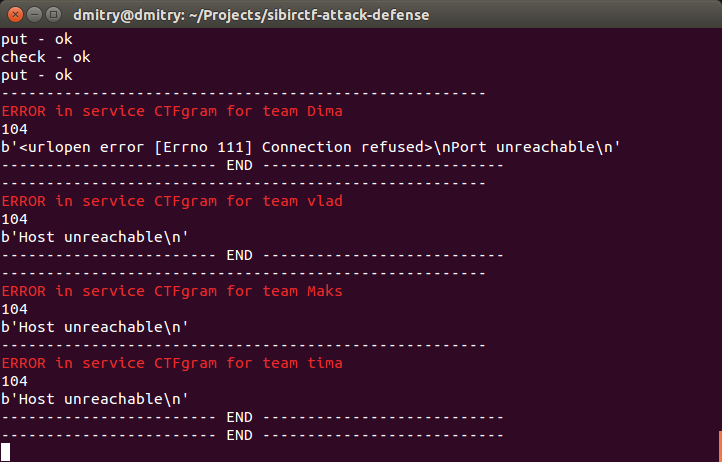
\includegraphics[width=1\linewidth]{images/round_sample.png}}
\caption{Пример вывода в консоль информации о работе модуля}
\end{figure}

\clearpage



Число 101 соответствует успешной работе сервиса команды-участника. Число 102 означает, что сервис команды работает, но на каком-то этапе отвечает некорректно. Число 103 означает, сервис команды отвечает, но не работает из-за какой-либо ошибки. Число 104 означает, что сервис команды не отвечает на запрос. 

Если на каком-то этапе <<чекер>> возвращает число отличное от 101, то дальнейшее выполнение программы прекращается. А статус <<чекера>> записывается в базу данных.

На 1 этапе каждому <<чекеру>> посылается адрес сервера команды-участника. 
На 2 этапе каждому <<чекеру>> посылается адрес сервера, идентификатор флага и сам флаг. 
На 3 этапе каждому <<чекеру>> посылается адрес сервера, идентификатор флага и сам флаг.

\begin{figure}[h!]
\center{\includegraphics[width=0.15\linewidth]{images/module_round_toservice.png}}
\caption{Блок-схема работы с каждым сервисом каждой команды-участника}
\end{figure}
\clearpage

Для увеличения производительности, каждый опрос сервисов команд-участников помещается в новый поток. Это позволяет работать в асинхронном режиме. Поэтому нестабильная работа сервиса команды-участника или ошибка в работе <<чекера>> не повлияет на опрос других сервисов. Также каждому потоку задается ограничение по времени работы. Это позволяет своевременно завершать процессы, тем самым уменьшается нагрузка на процессор и на потребление памяти.

